\chapter{Architecture}

The Flutter framework is organized into a series of layers, with each layer building upon the previous layer\\\\
\begin{figure}[h]
  \begin{center}
  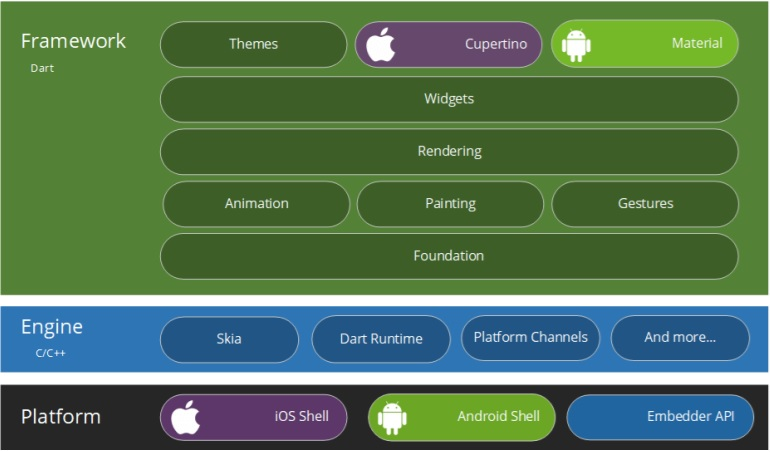
\includegraphics[height=80mm]{Images & Logos/CH_02_architecture.jpg}
  \end{center}
  \caption{Architecture of Flutter Framework}
\end{figure}\\  
  




\section{Dart Framework}

Flutter apps are created in the Dart programming language and take advantage of many of the language's more advanced features. Flutter operates in the Dart virtual machine, which contains an in-the-moment execution engine, on Android, as well as Windows, macOS, and Linux via the semi-official Flutter Work area Embedding project. Flutter apps for iOS employ ahead-of-time (AOT) compilation due to App Store constraints on unique code execution.
The Dart stage's support for "hot reload," which allows changes to source documents to be injected into a running application, is a standout feature. Flutter extends this by providing support for stateful hot reload, which allows changes to source code to be reflected in the current application without needing a restart or any loss of state.

\section{Flutter's Engine}
Flutter's Engine, which is based on C++, supports low-level rendering with Google's Skia Graphics package. It also interacts with platform-specific SDKs, such as those provided by Android and iOS.
The Flutter Engine is a small runtime that makes it easier to create Flutter applications. Flutter's key libraries, such as activity and designs, file and network I/O, accessibility support, plugin architecture, and a Dart runtime and compilation toolchain, are all executed by it. Most developers will be familiar with Flutter through the Flutter Framework, which provides a cutting-edge, responsive framework as well as a diverse set of staging, design, and setup tools.



\section{Platform}
Flutter provides a Shell with the Dart Virtual Machine at the platform level. The Shell is platform agnostic, allowing access to local APIs and easing the creation of stage-ready content. There's also an embedder API, which lets you use Flutter as a library rather than a framework for executing apps. The Shells also aid in establishing contact with the appropriate IMEs and the framework's application lifecycle events.